\chapter{Large Sphere Experiment} %new name?
\label{chap:LargeSphere}

\textit{The work presented here has been presented as an oral presentation at AIC 2013 \citep{macdonald_chromatic_2013} \textbf{prior to the author's involvement}, and as an oral presentation at ICVS 2017 \citep{garside_investigations_2017} by the author.}

Code and data is provided: \url{https://github.com/da5nsy/LargeSphere}

\section{Summary}

The goal of this experimental work was to examine the effect of different wavelengths of light upon chromatic adaptation. Our hypothesis was that \gls{ipRGC} stimulation may need to be considered in order to fully model the induced adaptation, with the null hypothesis being that chromatic adaptation can be fully accounted for by cone and rod mechanisms.

Within a Ganzfeld viewing environment, illuminated by one of 16 different wavelengths of near-monochromatic light, observers performed an achromatic setting task, controlling the chromaticity of a display visible in the central field through a 4$^{\circ}$ circular aperture with two handheld sliders.

\hl{Results:}

This project was designed before the author arrived at \gls{UCL}, and data from two participants had already been collected. Data collection required at least 16 hours commitment from observers, and so the only observers up to that point had been LM (one of the authors academic supervisors), who initiated the experiment, and TR who was a student of LM's. The original goal for my involvement in this project was that I should be a third observer, and assist in the data analysis. However, following the collection and initial data analysis of my own data, it appeared that there had been a technical fault during this run of data collection, and my data was deemed corrupted. %This data is discussed further in Appendix X. %%%%%%%%
Thus, my only contribution to this work is an extension to the data analysis started by LM, upon which I shall focus on in this chapter.

\section{Methodology}

\subsection{Hardware}

A hollow fibreglass sphere of approximately 750mm diameter was prepared with three holes; the first for an observer's face, the second (above) for an illuminant to illuminate the Ganzfed, and the third (opposite the first) through which a small portion of an LCD screen could be seen. The interior of the sphere was painted with RAL 7040 dulux vinyl matt, of approximately 38\% reflectance. Illumination was provided by a Kodak slide projector, filtered through one of 16 near-monochromatic filters, ranging in 20nm intervals from 400-700nm inclusive. % Add something about `mesopic'

\begin{figure}[htbp]
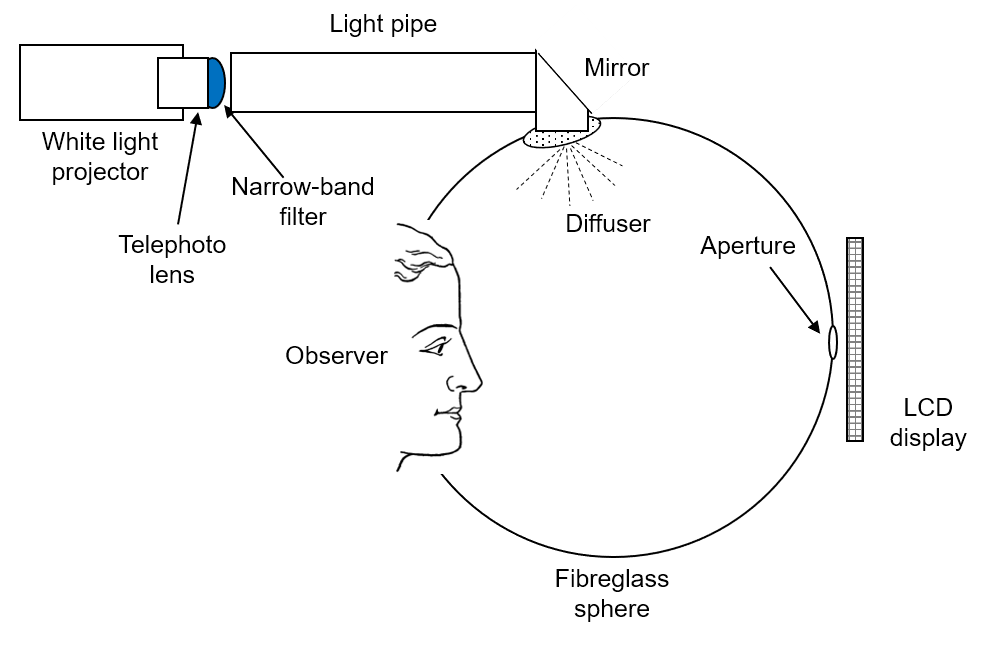
\includegraphics[max width=\textwidth]{figs/LargeSphere/sketch.png}
\caption{The hardware design. Illustration courtesy of Lindsay MacDonald.}
\label{fig:sketch}
\end{figure}

\begin{figure}[htbp]
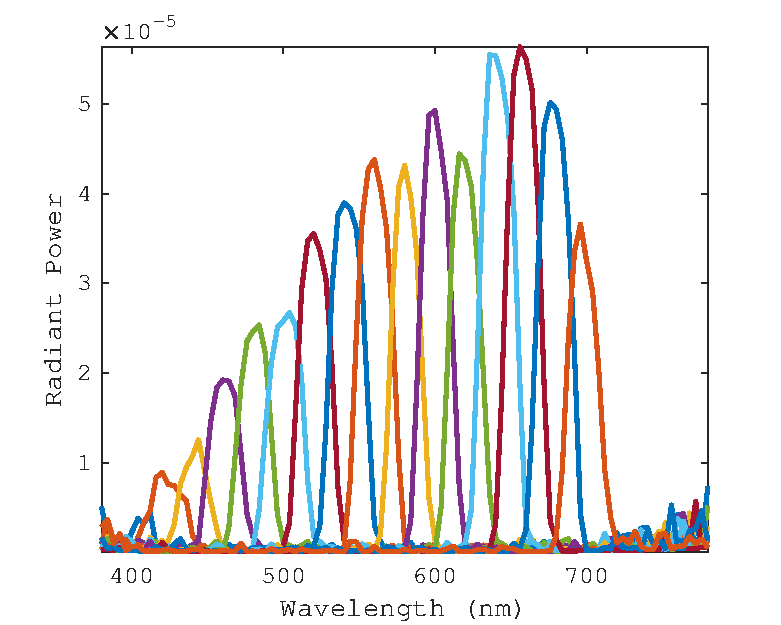
\includegraphics[max width=\textwidth]{figs/LargeSphere/LSillum.pdf}
\caption{The illuminants within the sphere, created by filtering light from a slide projector, measured as reflecting from a point just to the right of the aperture through which an observer would view the screen. Measurements made by Lindsay MacDonald.} %%%%%%?????
\label{fig:LSillum}
\end{figure}

\subsection{Observer task}

The observer sat on one side of the sphere with their face inside the sphere, such that nothing outside of the sphere was visible. On view on the opposite side of the sphere was a circular 4$^{\circ}$ aperture onto an LCD screen, upon which a random colour % drawn from ??????
was visible (See section \ref{sec:LSstim}). It was the observer's task to use two handheld sliders, which controlled the chromaticity of the screen, to make the appearance of the screen achromatic (an achromatic setting task). Once they were happy with the achromacy of the patch, they were to hit a button at which point a new random colour would be presented. The first displayed colour was displayed at L* of 85, with subsequent colours descending by 5 L* until 10 L*. This scale was repeated 10 times per session. Per session observers made 10 selections at 16 lightness levels (160 total). Observers performed 16 sessions (2560 selections total), visualised in Figure \ref{fig:ExperimentalPro}.

\begin{figure}[htbp]
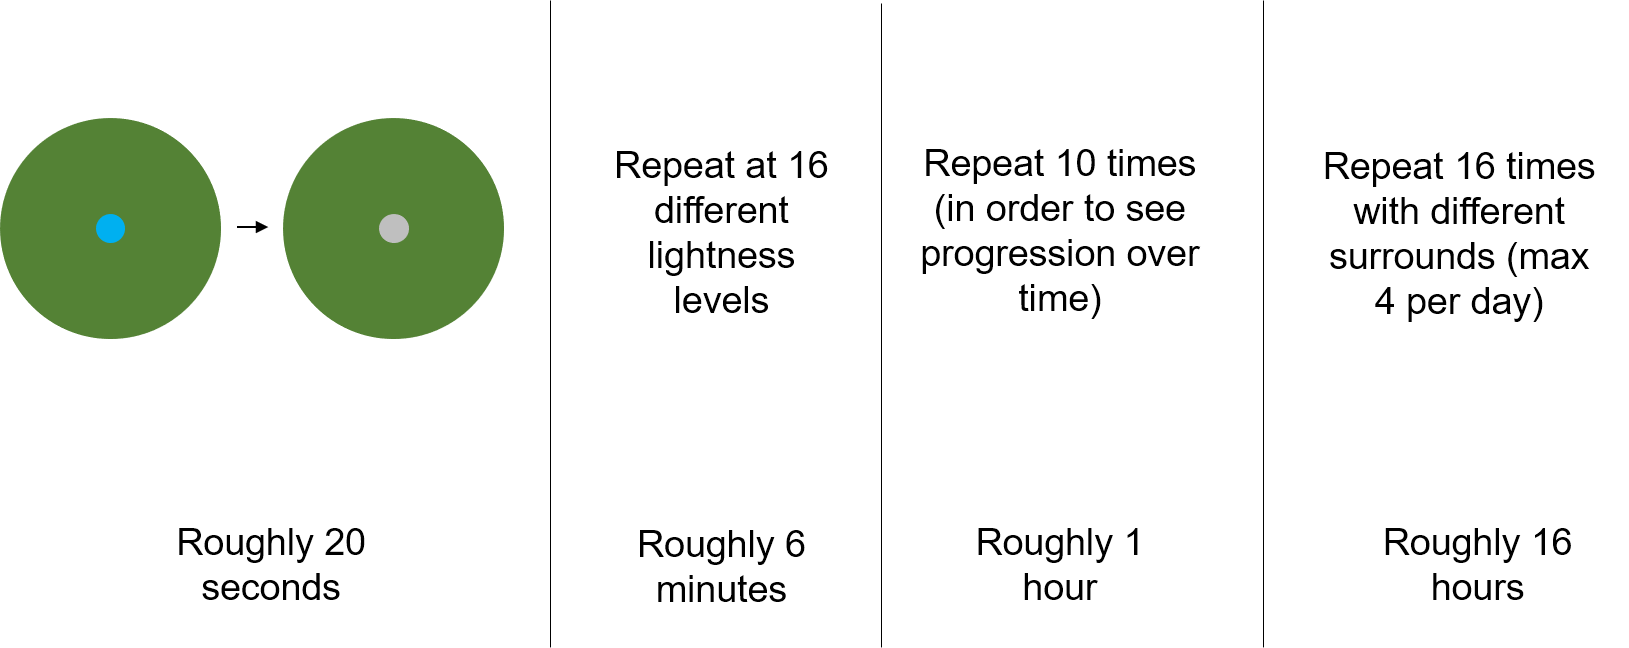
\includegraphics[max width=\textwidth]{figs/LargeSphere/ExperimentalPro.png}
\caption{The experimental protocol.}
\label{fig:ExperimentalPro}
\end{figure}

\subsection{Stimulus specification}
\label{sec:LSstim}

The stimulus was controlled via a MATLAB script, which read the input of two sliders and a button via a `Phidget' interface. The two linear sliders provided values of between 0 and 1000, and these values were converted to CIELAB co-ordinates in such a manner that the slider maxima corresponded to the Natural Colour System (NCS) unique hue positions as computed by \citet{derefeldt_transformation_1986}. In this manner the sliders could be considered as moving between red and green (via the CIELAB origin), and blue and yellow (via the CIELAB origin) respectively. These values were transformed into standard sRGB values, with white references of [XYZ = 99.04, 100, 151.30] for observer LM and [XYZ = 94.97, 100, 98.15] for observer TR, and these values were output to the screen.

The generation of random colours was achieved by modulating the nominal zero-point on each slider scale, where the default zero point is considered as 500, sampling from a uniform distribution between 250 and 750 for each presentation. 

The slider position was then considered relative to this new zero-point, meaning that once an observer hit the button to confirm their selection, a new random colour, anchored to their previous selection (in a rough manner) would be presented. It should be noted that this new colour was not entirely independent of the previous selection, due to this anchoring.

% \subsection{Data Collection}

% Data was collected for two observers \dots

\subsection{Data Processing}

Data were calibrated in the following manner: the recorded RGB values of the observers' selections were bounded (values above 1 or below 0 were brought within range, with an `absolute' rendering intent), quantized to 8-bits, and converted via look-up-table to \gls{CIE} 1931 XYZ tristimulus values. From these, xy chromaticities and CIELAB values were computed (with the white point of the display, as loaded from the characterisation file, used as the white reference).

A set of data referred to as the `baseline' data was generated, where there was no observer input, to consider the range of possible responses that an observer could make. This data was processed in exactly the same manner as the observer data, and is shown in Figure \ref{fig:overviewBL}, where it can be seen that the chromatic gamut increases as L* increases (due to a factor \texttt{cfac} in the display code which aimed to scale chromatic space with L*, mirroring the shape of CIELAB). It can also be seen that the gamut boundary is sometimes reached at higher levels of L*, with some of the vectors curving to remain within gamut.

\begin{figure}[htbp]
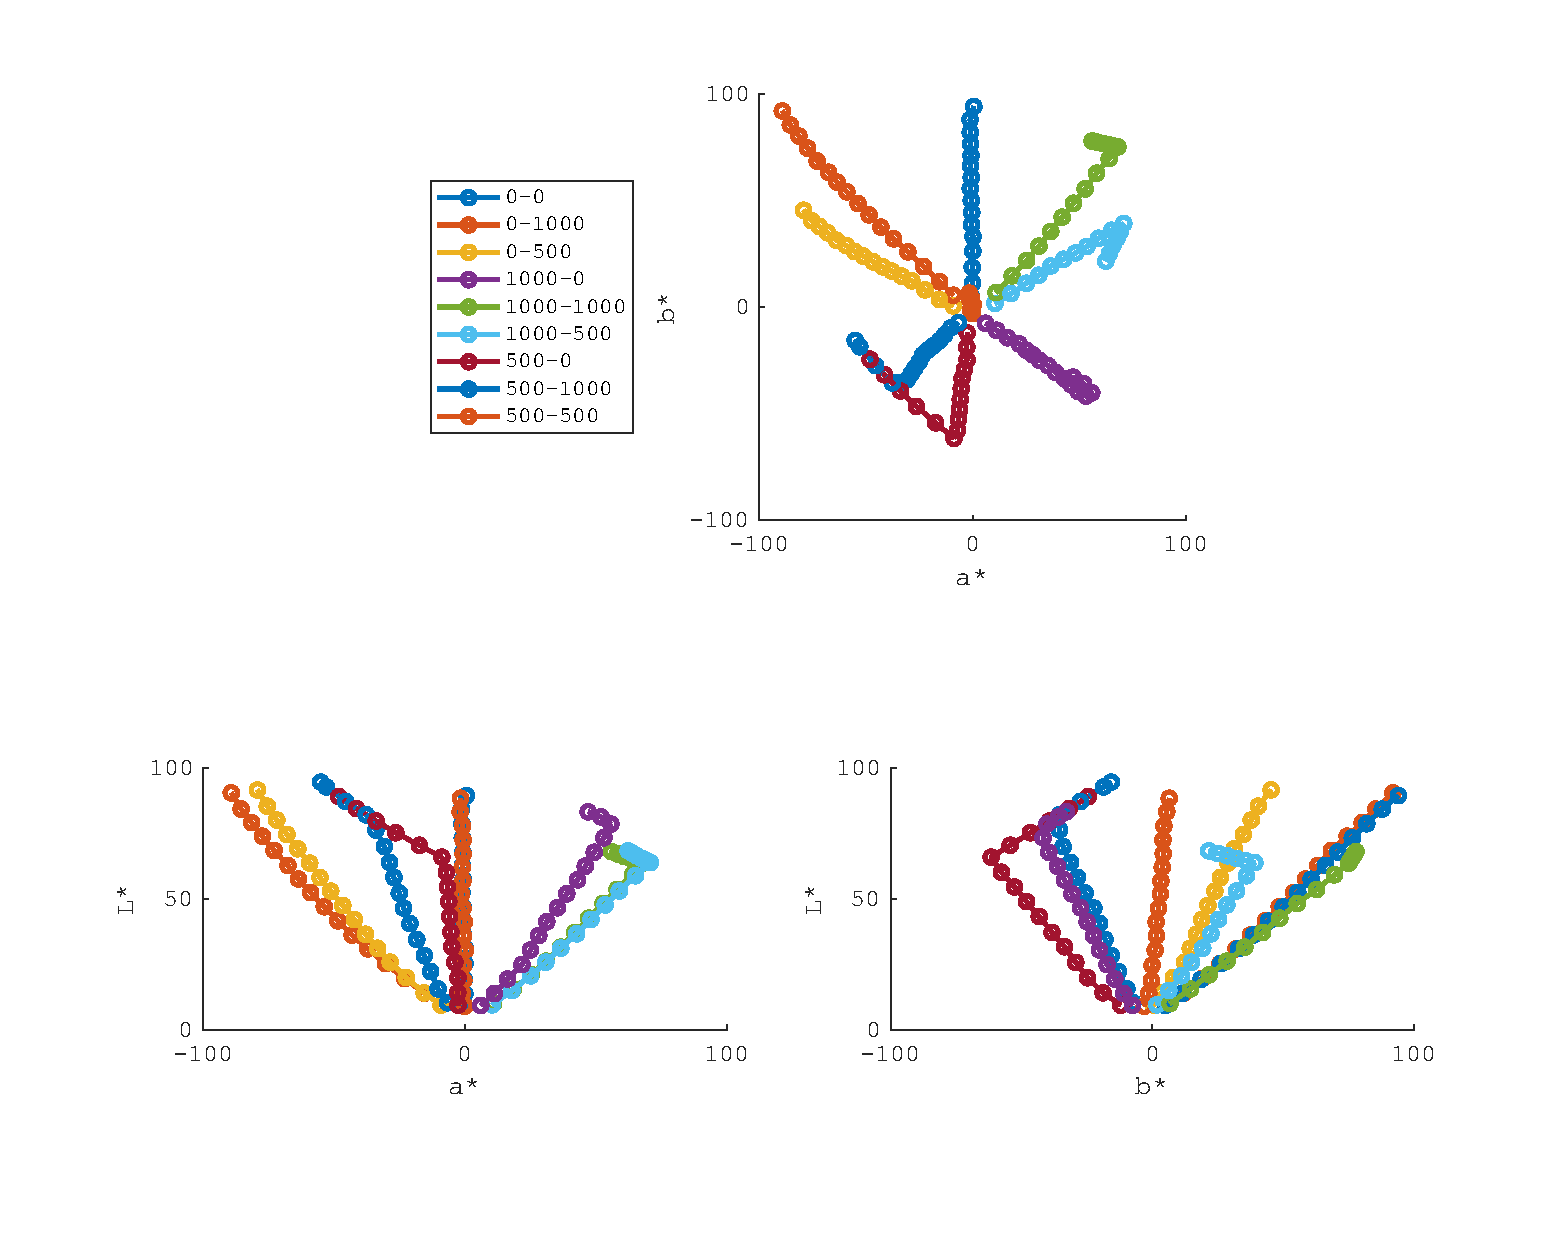
\includegraphics[max width=1.2\textwidth, center]{figs/LargeSphere/baselinedataOverview.pdf}
\caption{The baseline dataset. This data represents the condition where there is no observer input, and the two sliders are left at their maximum (1000), minimum (0), or neutral (500) positions (9 combinations). In the legend the first number denotes the slider A position, and the second denotes the slider B position.}
\label{fig:overviewBL}
\end{figure}

%The effect of the random offsetting was also queried, and it was found that the maximum random offset pushed the chromaticities halfway between \dots

Two distinct approaches were taken to data analysis. The first attempted to process the data in a chromatic space, with the reasoning that under the null condition chromatic selections should simply correspond to the chromaticity of the surround illuminants, presumably with some sort of gain function applied. If it were shown that this relationship was not as expected, in a manner which might suggest involvement by other mechanisms (meaning rods or \glspl{ipRGC}), then this could be considered as evidence against the null hypothesis.

The second approach took advantage of the fact that measurements were taken at samples across the wavelength spectrum. Since we know the power at each waveband, and the spectral sensitivities of the receptors, we can see whether the responses (transformed to cone space) relate in some simple way to spectral sensitivities.

%Here the logic was that if the null condition were true, we should be able to fit a model to observer responses which only used cone-based inputs, and we could carefully consider the (presumed) benefit of including rods and \glspl{ipRGC} in the model. If either rod input or \gls{ipRGC} input were found to dramatically improve the model then this could be considered as evidence against the null hypothesis.

\section{Results}

\subsection{Summary}

Visually summarising the results for even a single observer is difficult due to the high number of variables and collected datapoints. In the following plots data is averaged over the 10 runs within each session (under each adapting wavelength). In Figures \ref{fig:overviewLM} - \ref{fig:overviewDG} data from LM, TR and the author (DG) is presented.

\begin{figure}[htbp]
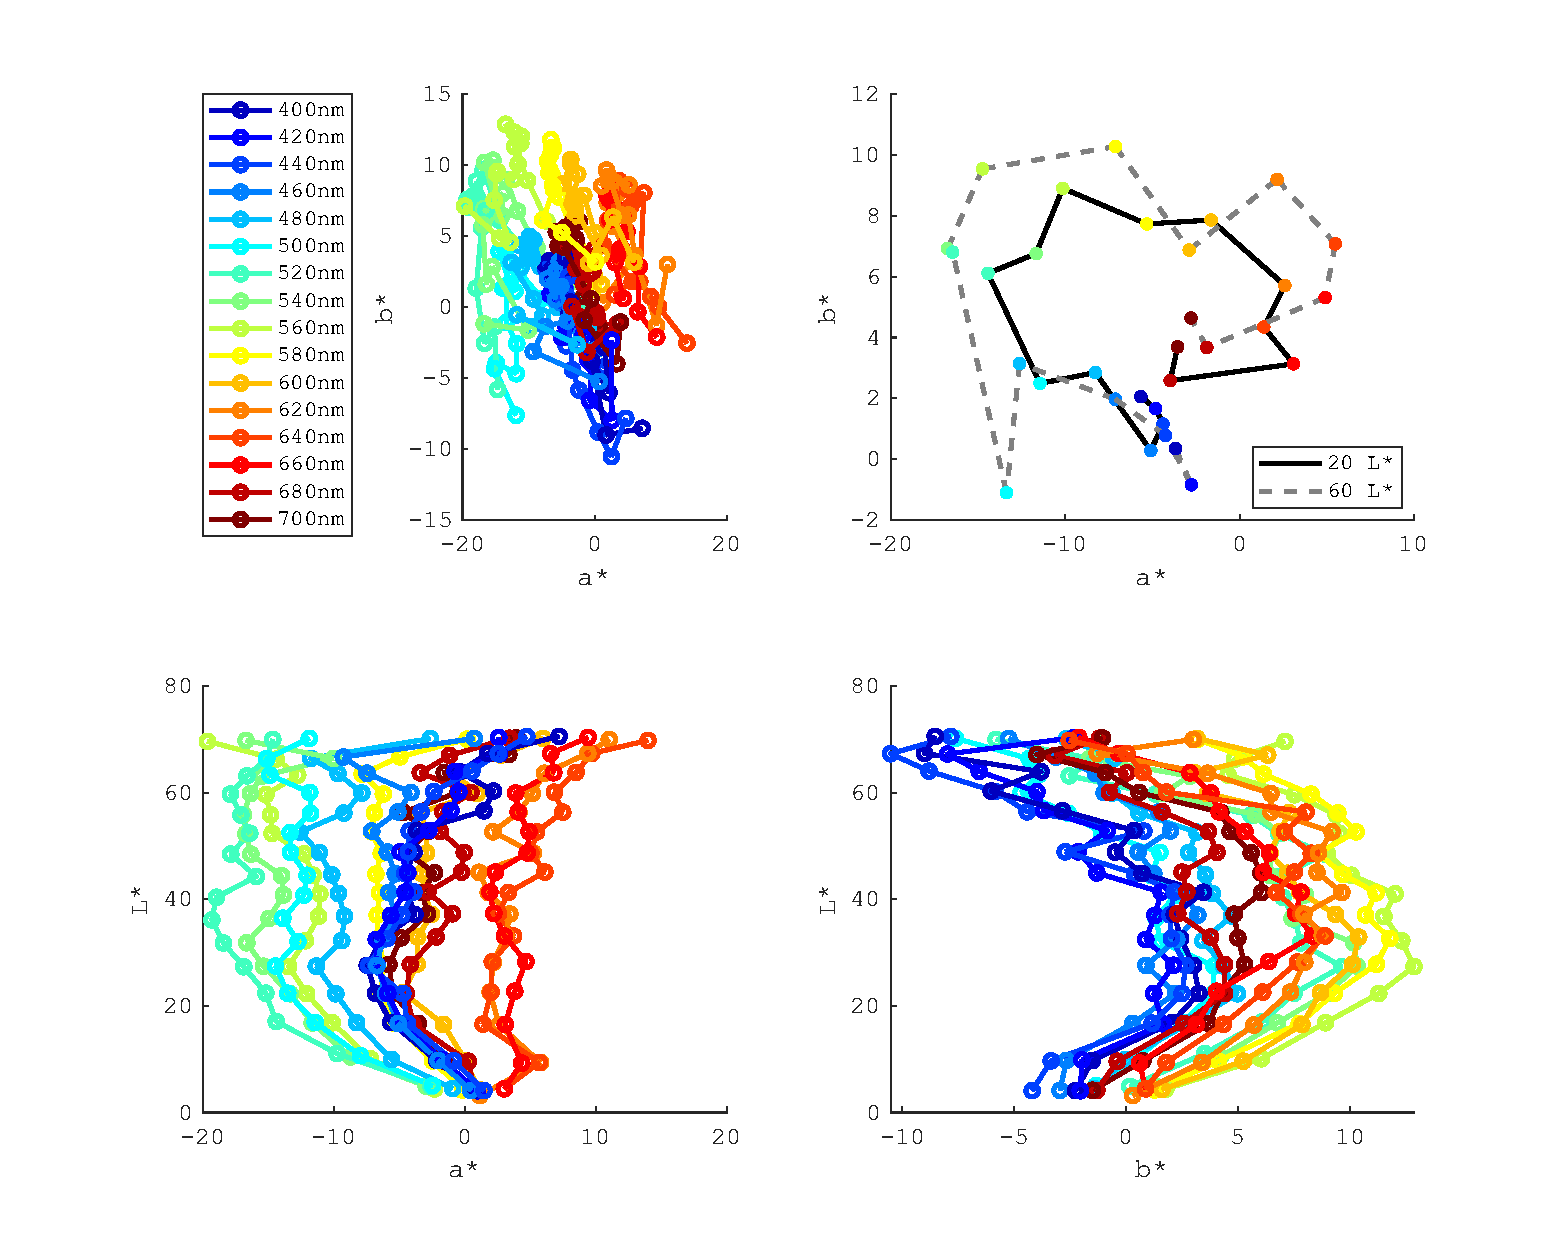
\includegraphics[max width=1.2\textwidth, center]{figs/LargeSphere/LMdataOverview.pdf}
\caption{The dataset of observer LM. In all plots, the average CIELAB values are taken over the 10 repeats within each session. \emph{Top left:} an overview of the chromaticity of selected points. Connections between points indicate that they are from the say run (under the same adapting wavelength). Colouring of points and lines indicates the adapting wavelength. Whilst there is a rough correspondence between the colour of the line and the appearance of the adapting field this is only meant as a means to differentiate between the different lines. \emph{Top right:} as for top left but only for points recorded at specific values of L*. Colours are as for top left, but lines linking points now represent points of like L*. This plot is included to show the relationship across wavelength of the adapting field. \emph{Lower left and right:} Other perspectives upon the CIELAB projection. Data as for top left.}
\label{fig:overviewLM}
\end{figure}

\begin{figure}[htbp]
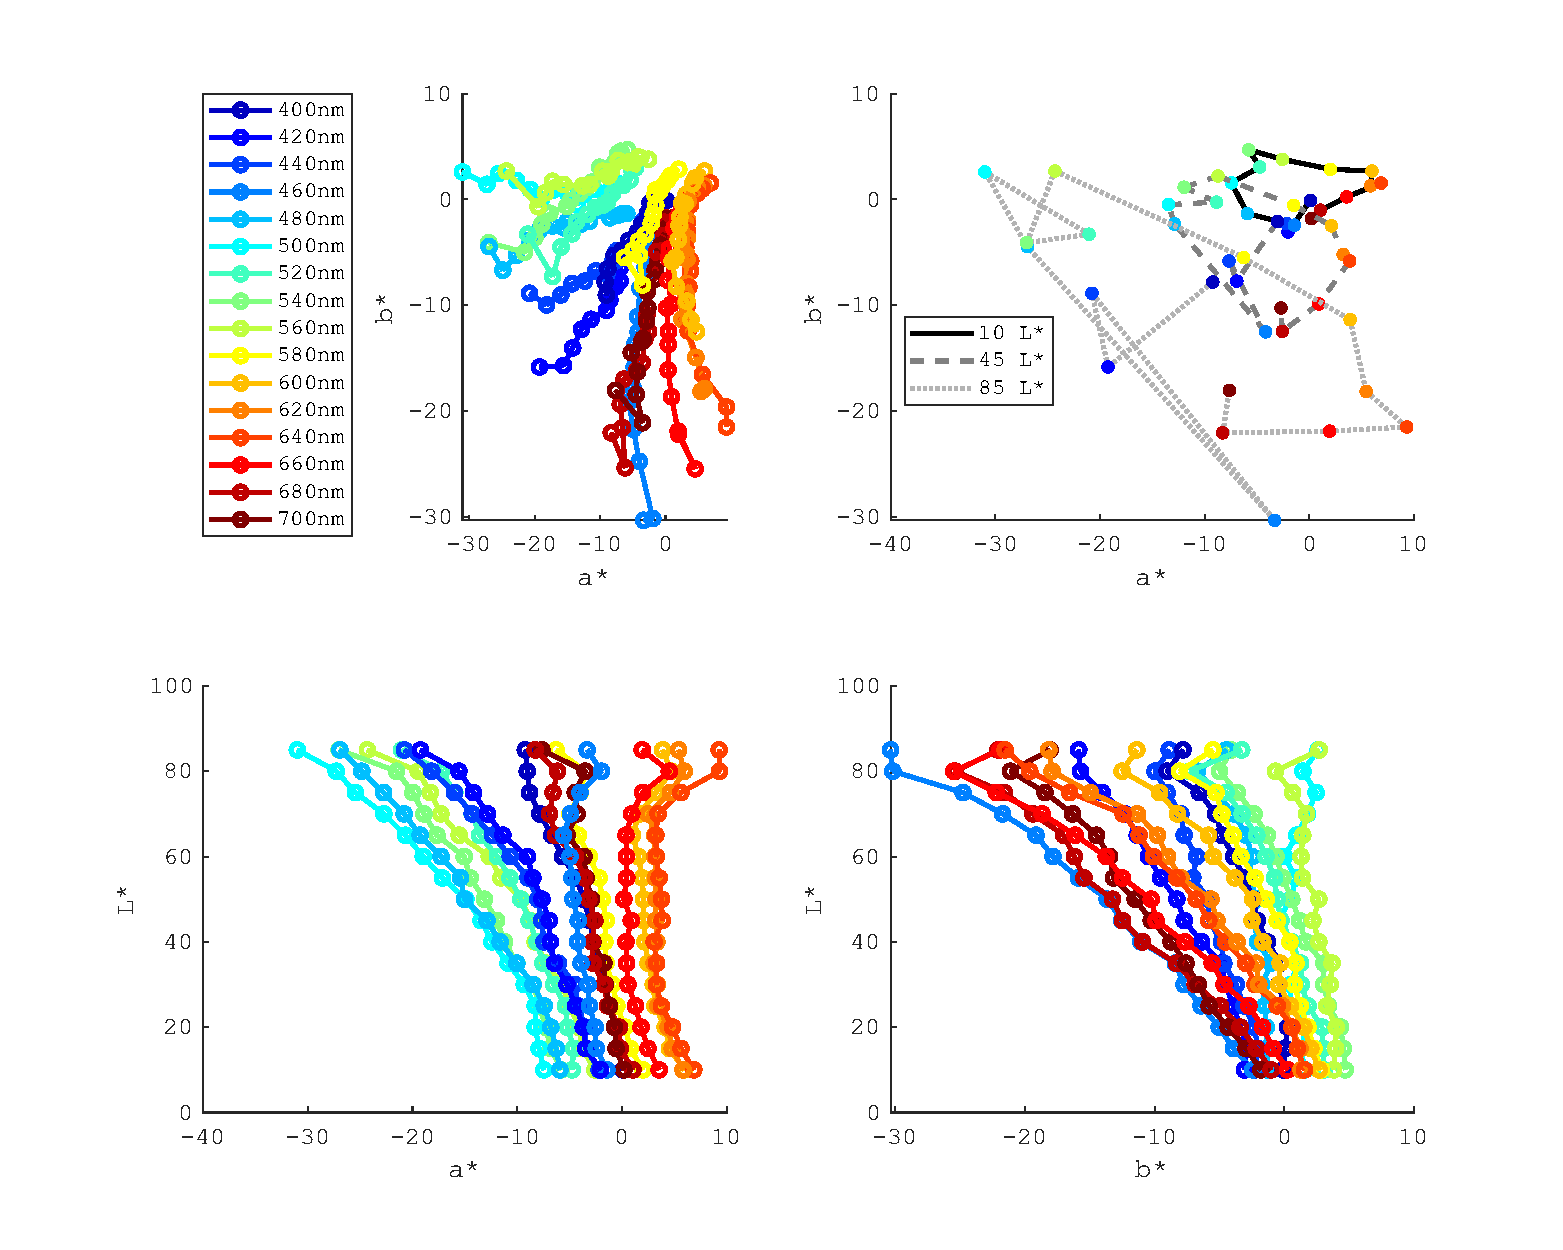
\includegraphics[max width=1.2\textwidth, center]{figs/LargeSphere/TRdataOverview.pdf}
\caption{As per Figure \ref{fig:overviewLM}, but with the data of observer TR.}
\label{fig:overviewTR}
\end{figure}

\begin{figure}[htbp]
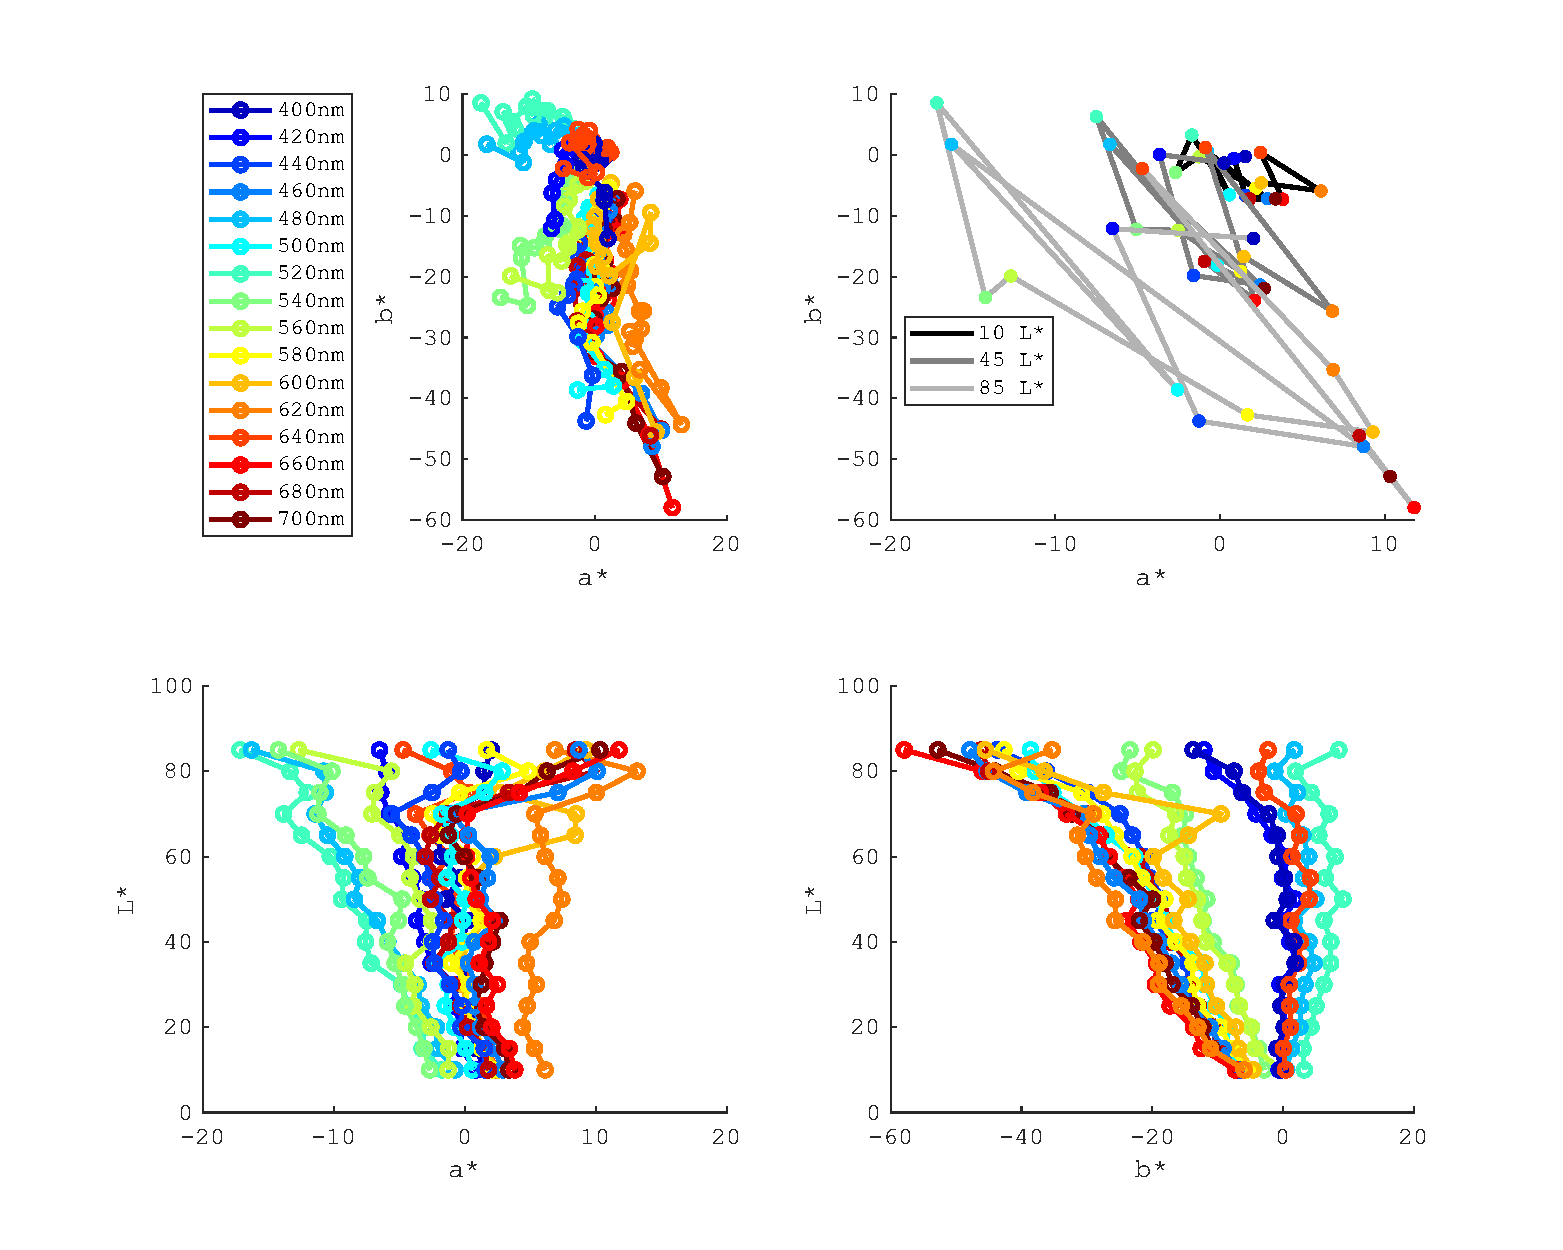
\includegraphics[max width=1.2\textwidth, center]{figs/LargeSphere/DGdataOverview.pdf}
\caption{As per Figure \ref{fig:overviewLM}, but with the data of observer DG.}
\label{fig:overviewDG}
\end{figure}

It can be seen in the data for all observers that there is a clear L*-dependent shift. Interestingly, the precise nature of this seems different for each observer; the data of LM clusters tightly around [0,0] for low values of L* and then generally moves north-west as L* increases, before returning towards the origin at the highest values of L*. For TR the shift is monotonic and roughly south-west.

Within this pattern it can be seen for observers LM and TR that there is a correspondence between the adapting wavelength and the selected chromaticity. This is most easily seen in the top right plots of Figures \ref{fig:overviewLM} and \ref{fig:overviewTR}. In both cases a rough circle can be seen for both of the values of L* shown.

In Figure \ref{fig:overviewDG} is can be seen in the lower-right plot that the data splits into two distinct groups, one is which is considerably lower in b* than is seen for either of the previous observers, or would generally be expected. It is suspected that there was a screen calibration issue which led to offsetting of the screen output in an unpredictable session-by-session fashion. It was found that a basic offsetting applied selectively to those sessions which appeared to be affected could `correct' for this issue, but without a better understanding of the issue this dataset is considered unsuitable for further analysis.

\subsection{Variability over time/repeats}

Not represented in the above plots is the way in which responses varied over time within each session, averaged over L* (the previous plots were averages over time). Figures \ref{fig:timeLM} and \ref{fig:timeTR} show the calibrated CIELAB values for observers LM and TR. 

L* should theoretically remain steady throughout, with minor differences introduced presumably due to differences between the screen and sRGB, 8-bit quantization, and any selections where a gamut boundary was reached. Both a* and b* follow the broad trends which would be expected given previous figures. Newly visible in these figures is the manner in which responses change over time. For both observers LM and TR the first two or three repeats seem to be distinct from the rest of the set, suggesting that adaptation had not yet reached a steady-state during this time.

\begin{figure}[htbp]
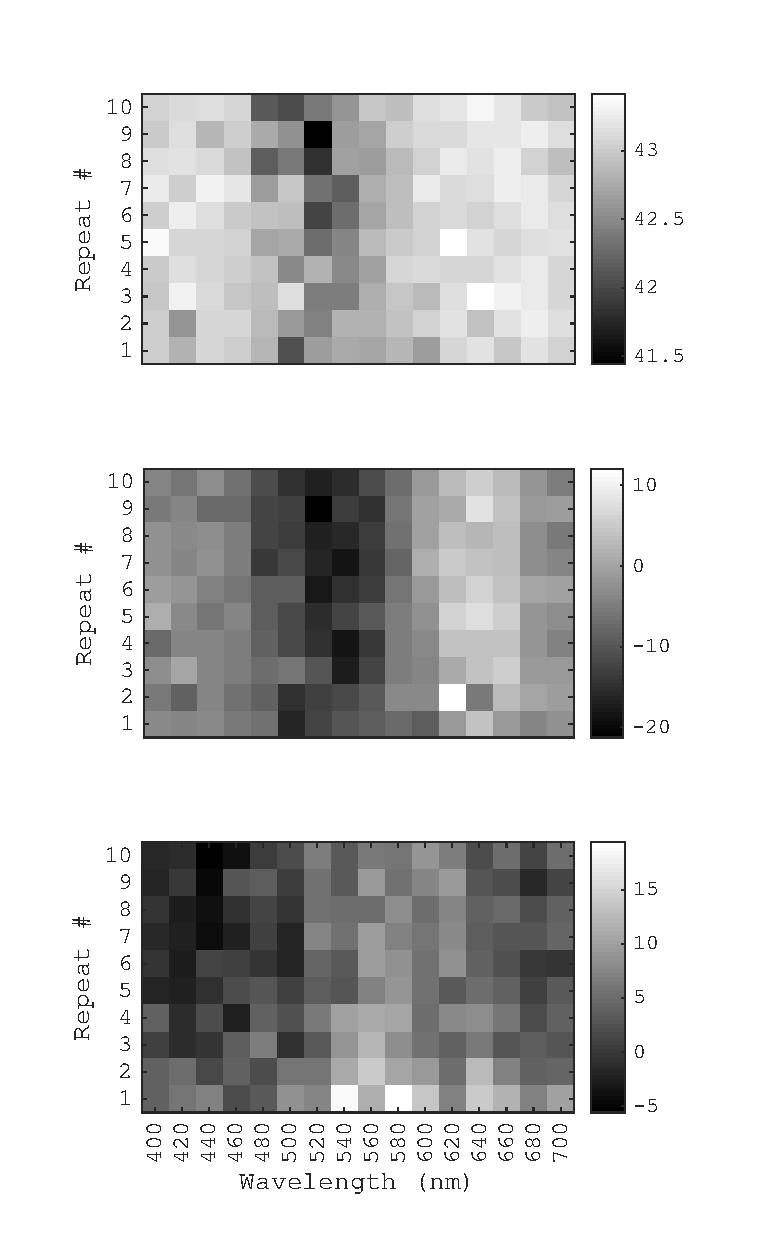
\includegraphics[max width=1.2\textwidth, center]{figs/LargeSphere/LMdataOverTime.pdf}
\caption{CIELAB co-ordinates across time (repeat #). Top plot is L*, middle a* and lower b*.}
\label{fig:timeLM}
\end{figure}

\begin{figure}[htbp]
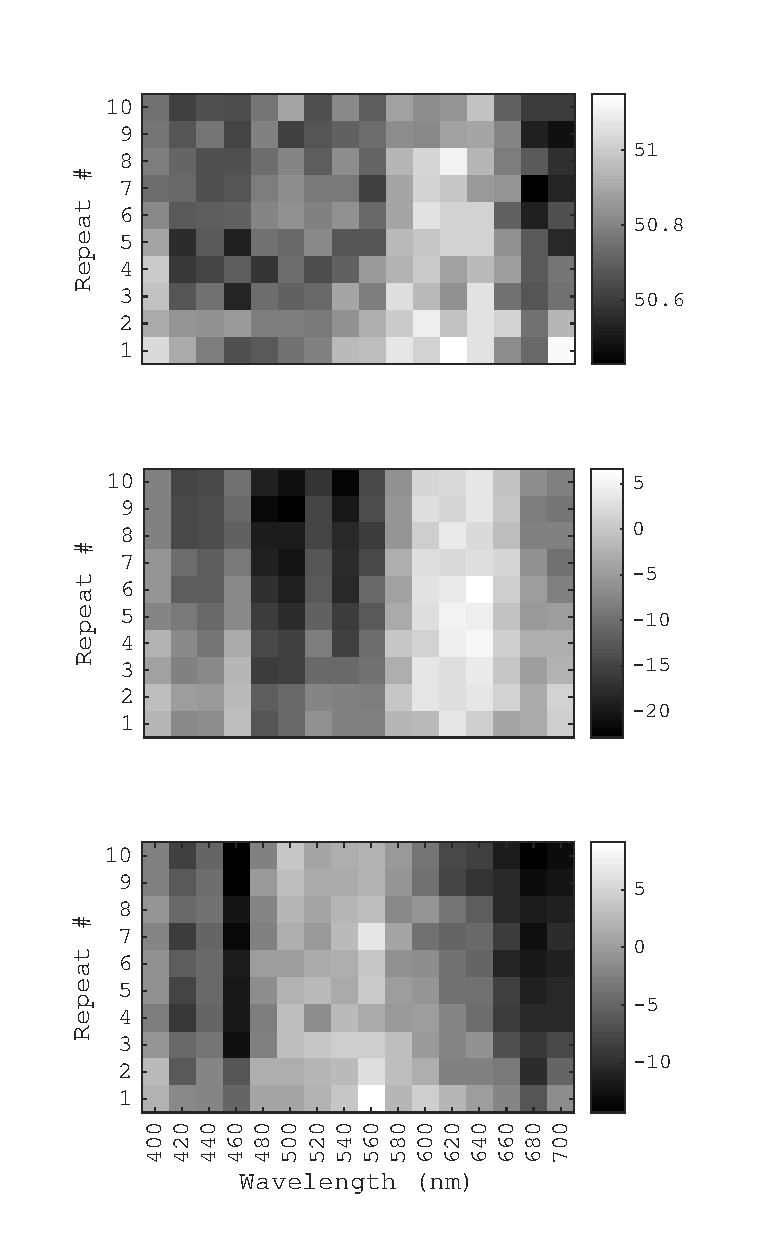
\includegraphics[max width=1.2\textwidth, center]{figs/LargeSphere/TRdataOverTime.pdf}
\caption{As per Figure \ref{fig:timeLM}, but with the data of observer TR.}
\label{fig:timeTR}
\end{figure}


\clearpage


\subsection{Chromaticity-based analysis}

The CIELAB co-ordinates for the adapting fields were computed from the measurements shown in Figure \ref{fig:LSillum}, relative to the white point of the display, and are presented in Figures \ref{fig:adapter1} and \ref{fig:adapter2}. 

\begin{figure}[htbp]
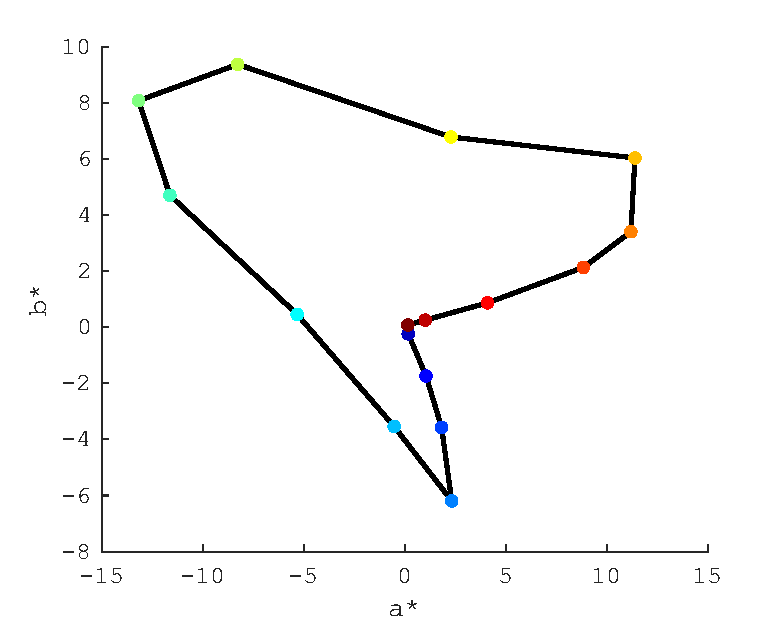
\includegraphics[max width=\textwidth]{figs/LargeSphere/adapter1.pdf}
\caption{The CIELAB values for the surround illuminants, calculated from the measurements shown in Figure \ref{fig:LSillum}, taking the white point of the screen as the white point.}
\label{fig:adapter1}
\end{figure}

\begin{figure}[htbp]
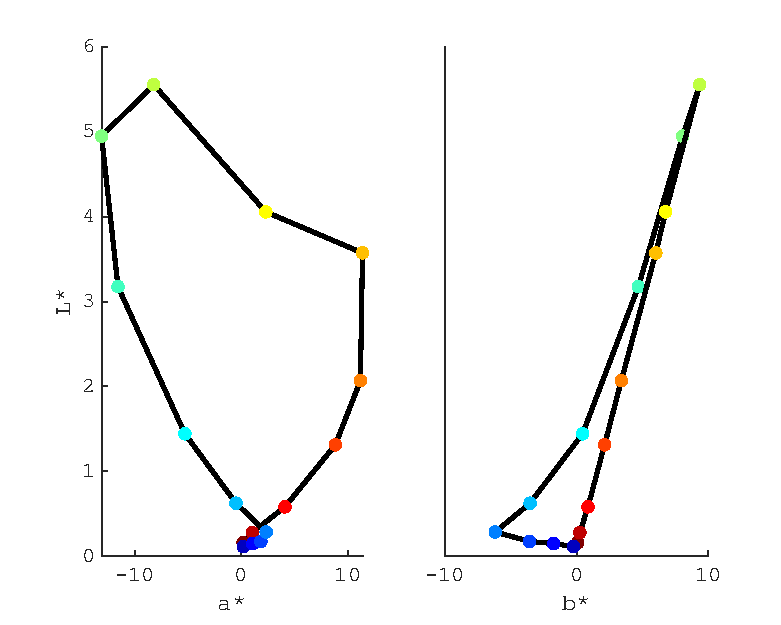
\includegraphics[max width=\textwidth]{figs/LargeSphere/adapter2.pdf}
\caption{As per Figure \ref{fig:adapter1}, but different perspectives upon the three-dimensional CIELAB space.}
\label{fig:adapter2}
\end{figure}

If we were to assume a very basic adaptive system, and the full validity of CIELAB as a model of visual processing, then we might expect to see something which mirrors this pattern. Observer TR's data exhibits a trend roughly similar to this; a roughly circular plot in the top right of Figure \ref{fig:overviewTR}.

Observer LM's data however, does not resemble this pattern. %DG's data, well, the less said the better.

Considering that there is a clear L*-dependent shift in chosen chromaticities (though I don't know how much of this is dependent upon the chroma shift added to the stimulus with the experiment, and I don't know how much the different in results is due to the different white points for the two observers).

\subsection{Spectrum-based analysis}

\textit{The code to reproduce the following analysis can be found at \url{https://github.com/da5nsy/LargeSphere/blob/master/Data\%20Analysis/VonKriesTest.m}}

The first stage of this analysis was to generate simulated data which represented the situation whereby there was only simple Von Kries adaptation. This was accomplished by multiplying the individual \glspl{SPD} (Figure \ref{fig:LSillum}) by the CIE 2006 10$^{\circ}$ observer fundamentals (not in the manner in which this is usually done, resulting in tristimulus values, but rather point-wise, thus retaining the spectral nature of the data). See Figure \ref{fig:LSsimdata}.

\begin{figure}[htbp]
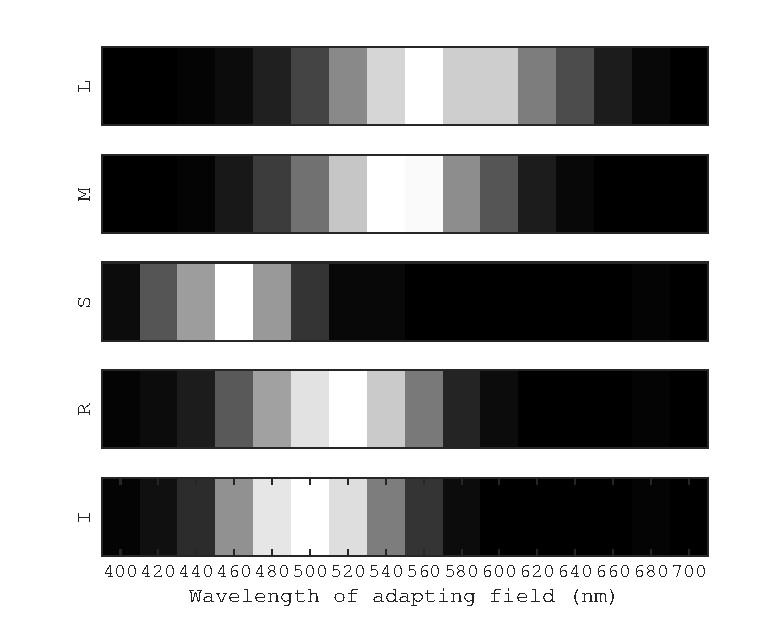
\includegraphics[max width=\textwidth]{figs/LargeSphere/LSsimdata.pdf}
\caption{Simulated data for a basic Von Kries observer. In this figure white represents a high response. For example, with 560nm peripheral stimulation we would expect an observer to pick a colour with high L-cone activation as achromatic, assuming that the sensitivity of L-cones had been suppressed and thus higher activation was required to reach a neutral point (see peak roughly in the centre of the top bar).}
\label{fig:LSsimdata}
\end{figure}

A comparison was then made between this data and a set of real data (Obs = TR, averaged over time (entire run, no exclusions), averaged over L* = 35:60). This real data had been transformed from the recorded RGB values of achromatic matches into LMS values. It can be seen that there is a considerable difference between the simulated data and the real data (Figure \ref{fig:simVreal}). S-cone data shows the closest match, with the predicted peak at 460nm\footnote{Note that this is not at the peak sensitivity of s-cones (which would appear at 440nm for this dataset at 20nm intervals) but rather at the peak of the s-cone sensitivity function multiplied by the \gls{SPD}, as plotted in Figure \ref{fig:LSsimdata}.} being mirrored in the real data. This peak appears to bleed into the (real) M-cone data, and the simulated data for L and M-cone data shows very little correspondence to the collected data. Correlation coefficients between the simulated and this specific real dataset are 0.1399, -0.2509, 0.3164 for L, M and S respectively.

\begin{figure}[htbp]
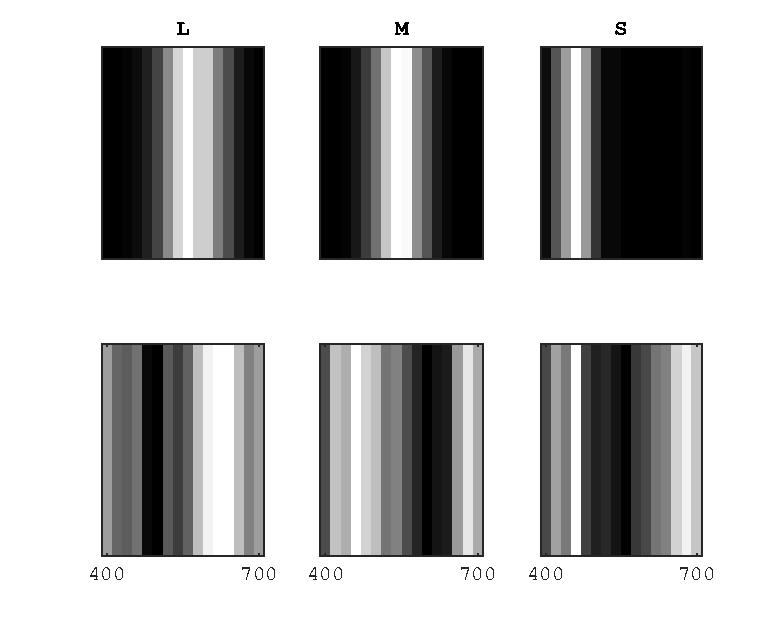
\includegraphics[max width=\textwidth]{figs/LargeSphere/simVreal.pdf}
\caption{A comparison of simulated data (top row) and real data (bottom row). Data from the top row is as per the top three bars of Figure \ref{fig:LSsimdata}.}
\label{fig:simVreal}
\end{figure}

In order to understand the way in which adaptation may be crossing between channels, or the way in which we may have not properly isolated our channels (it is unclear exactly how much freedom an observer truly has to move around the response space) a brute-force method was used to find combinations of the above simulated data which would best fit the real data.

10000 random sets of weighting values (30000 values total) between -25 and 25\footnote{An analysis showed that the absolute range of these figures was unimportant, since we were looking for correlation with the real data rather than absolute correspondence. Thus they are listed here only to assist the reader in understanding graphs such as Figure \ref{fig:contributions_3}.} were generated. These weightings were applied to the simulated responses and the results were additively combined\footnote{(X amount of simulated L) + (Y amount of simulated M) + (Z amount of simulated S)}. The correlation between this new random combination and each channel of the real data was computed. The top performing randomly generated combinations were selected and are presented in Figure \ref{fig:maxsimVreal}. These particular combinations were created through cross-combining the original simulated data (top row of Figure \ref{fig:simVreal}), in the ratios shown in Table \ref{tab:crosscomb} and correlated with the real data to extent of the following coefficients: 0.9126, 0.8861, and 0.7726 for L, M and S respectively. These are much improved over the coefficients for the original simulated data.


\begin{table}[hbtp]
\centering
\begin{tabular}{|r|r|r|r|}
\hline
 & L & M & S \\ \hline
L & $18.4069$ & $-23.2578$ & $-10.9817$ \\ \hline
M & $-13.0477$ & $9.8327$ & $10.6844$ \\ \hline
S & $-2.7633$ & $-17.6798$ & $8.3036$ \\ \hline
\end{tabular} % Would be nice to format to fit page width
\caption{Optimal weights to fit the specific real dataset used. \\ \emph{Example: Image in top left of Figure \ref{fig:maxsimVreal} (L) was created by combining 18.4069 * the original simulated L (Top left of Figure \ref{fig:simVreal}), -23.2578 * the original simulated M and -10.9817 * the original simulated S.}}
\label{tab:crosscomb}
\end{table}

\begin{figure}[htbp]
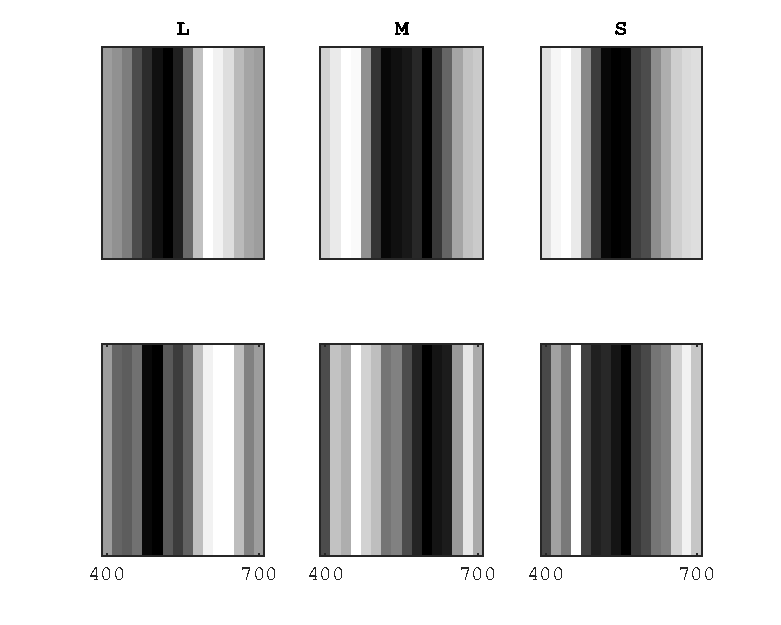
\includegraphics[max width=\textwidth]{figs/LargeSphere/maxsimVreal.pdf}
\caption{A comparison of randomly generated combinations (top row) whereby channels were freely mixed from basic Von Kries simulated data (top row of Figure \ref{fig:simVreal}) to best correlate with real data, and real data (bottom row) (repeated from Figure \ref{fig:simVreal}).}
\label{fig:maxsimVreal}
\end{figure}

\begin{figure}[htbp]
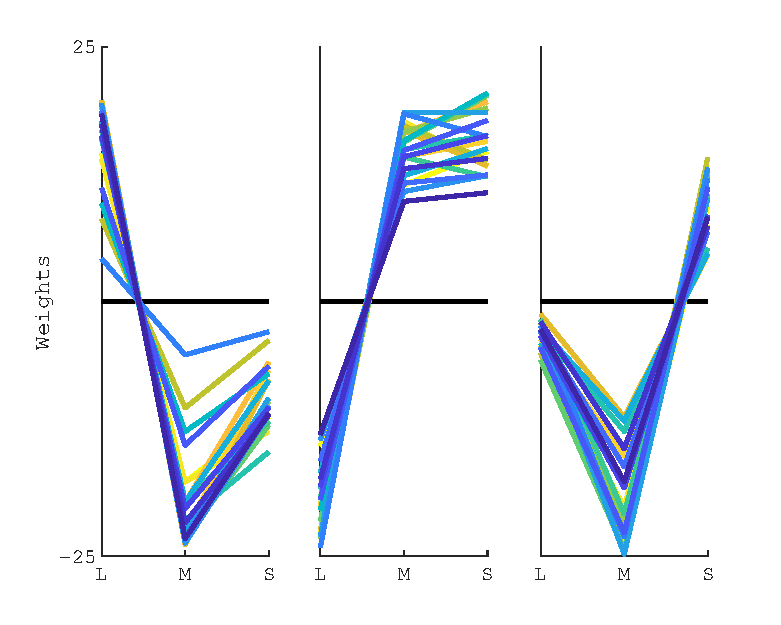
\includegraphics[max width=\textwidth]{figs/LargeSphere/contributions_3.pdf}
\caption{Top 0.2\% performing randomly generated combinations, presented in terms of the weights of the original simulated data that they use. The subfigure on the left represents the weights needed to reconstruct the real data for L, the middle - M, and the right - S. Colour coded such that dark blue is the highest performing and yellow is the worst performing (of this highly performing subset).}
\label{fig:contributions_3}
\end{figure}

\begin{figure}[htbp]
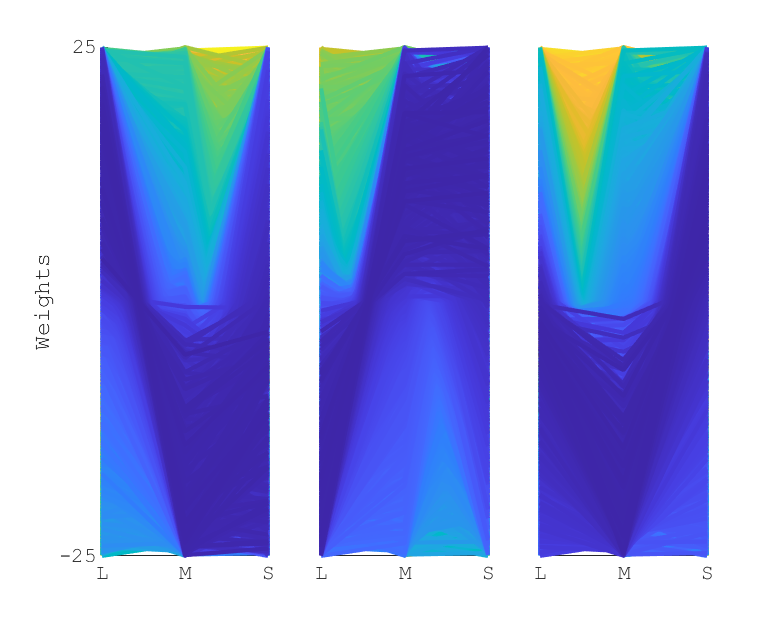
\includegraphics[max width=\textwidth]{figs/LargeSphere/contributions_all.pdf}
\caption{As per Figure \ref{fig:contributions_3} but for all randomly generated combinations. The trends seen in Figure \ref{fig:contributions_3} are visible, and the range of these trends (extending into the poorer performing randomly generated combinations) can be seen. The colours are rescaled such that yellow now represents the worst performing randomly generated combinations of the entire set. Plots are plotted ordered by success and so lines representing successful randomly generated combinations will overlay lines representing poorer performing ones.}
\label{fig:contributions_all}
\end{figure}

The top performing 0.2\% of the randomly generated combinations are presented in terms of their components (analogous to plotting the values in \ref{tab:crosscomb}) in Figure \ref{fig:contributions_3}, and the entirety of the results for the randomised sampling presented in Figure \ref{fig:contributions_all}. 

It can be seen that to reconstruct the real data for L, a high amount of simulated L, and a low amount of both simulated M and S are required, though from Figure \ref{fig:contributions_all} it can be seen that the requirement for low S is less stringent. It can also be seen that the amount of L required seems related to the amount of M required (from the way in which the lines cross at a point).

A similar but opposite trend is visible for M.

For S, there is a narrow range of successful values for L (negative but close to 0), a larger range of strongly negative values for M, and a range of positive values for S. The reciprocal relationship between L and M seen in the reconstructions of L and M is no longer visible, but instead there is a new reciprocal relationship visible between M and S, though examination of Figure \ref{fig:contributions_all} suggests that this is not as important as in the case of L and M.

It is reassuring that in each case, successful random combinations used high positive levels of the target signal. For both L and S the target signal was the only positive weighting, with M taking positive weights of both M and S. 

\subsubsection{Adding rods and ipRGCs}

In order to investigate whether rods or \glspl{ipRGC} were playing a role in adaptation as measured by this dataset, the analysis was re-run with the additional rod input, additional \gls{ipRGC} input, and both rods and \glspl{ipRGC} as additional inputs. See Figure \ref{fig:LSsimdata} for a visualisation of these channels. The results of re-running the computations following the addition of these inputs is shown in Table \ref{tab:plusres}. Minor increases in correlation are exhibited. However, it should be noted that one would expect to see at least a minor increase in ability from practically any additional signal, so long as it differed from the already accessible signals.

\begin{table}[hbtp]
\centering
\begin{tabular}{|r|r|r|r|}
\hline
Just cones: & $0.9126$ & $0.8861$ & $0.7726$ \\ \hline
+ rods: & $0.9156$ & $0.8881$ & $0.7987$ \\ \hline
+ ipRGCs: & $0.9218$ & $0.8867$ & $0.8055$ \\ \hline
+ rods + ipRGCs: & $0.9326$ & $0.8933$ &$0.8100$ \\ \hline
\end{tabular} % Would be nice to format to fit page width
\caption{Correlation coefficients for various conditions incorporating additional signals.}
\label{tab:plusres}
\end{table}

Further, it is not clear to what extent the gains exhibited in Table \ref{tab:plusres} are due to noise within the computations; the randomly generated combinations are set via a random number generator which is re-set each time the script is run for reproducibility, however there is nothing to stop the randomly generated values for the additional input runs performing better purely by chance alone. In order to investigate this, the above extensions were re-run 100 times each, and the top performance for each skimmed and saved. The results of this are presented in Figure \ref{fig:relcontributions}. From this figure it can be seen that there is a real and clear benefit from the inclusion of the additional signals, and from inclusion of \emph{both} of the additional signals.

\begin{figure}[htbp]
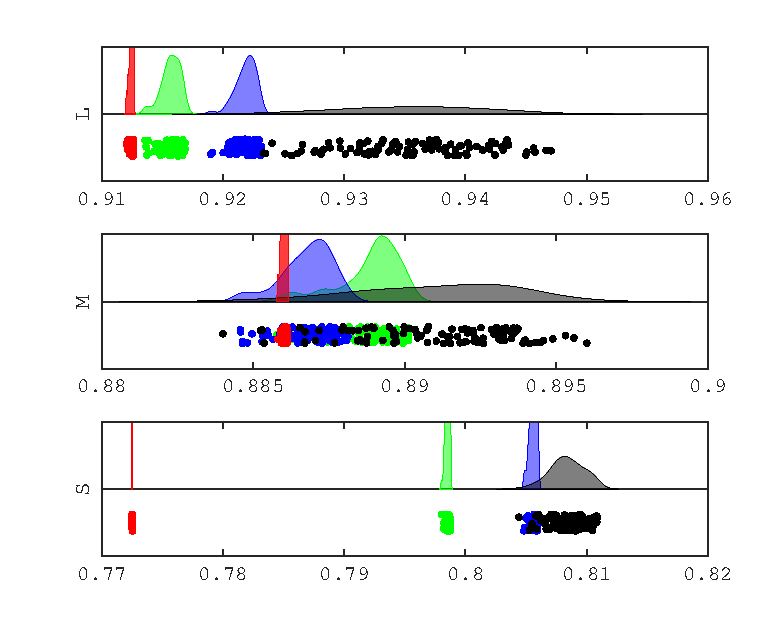
\includegraphics[max width=\textwidth]{figs/LargeSphere/relcontributions.pdf}
\caption{Raincloud plot \cite{allen_raincloud_2019} showing the results of re-running the extended analyses 100 times and skimming the best performer from each. Red points and probability density function represent `just cones', green - `+ rods', blue - `+ \glspl{ipRGC}', black - `+ rods + \glspl{ipRGC}'.}
\label{fig:relcontributions}
\end{figure}

\section{Discussion}

There is a clear distinction between the simple simulated response functions, and the recorded data. It is interesting that a simple linear recombination can improve the correlation so greatly. It should be remembered however that this type of post-hoc fitting is liable to delivering the results a researcher might hope to find. 

Taken at face value, the results seem to indicate that the principal drivers of adaptation are not at the cone level, but rather at a higher level, once cone inputs have been combined. The results mirror what might be expected of these higher level signals - there appears to be a single signal for L and M, roughly mirrored between the two, with a reciprocal trade-off possible between L and M for both, and the S cone signal takes positive weights for S, and negative weights for both L and M, but with a curious hint of a reciprocal trade-off between S and M.

However, it is unclear to what extent these relationships may arise due to limitations of the experimental set-up; it is possible that a rise in one signal is yoked through hardware limitation to the rise or fall in another. Future investigators should consider whether this effect is modellable.

\subsection{Additional Signals}

Though there is a demonstrated ability of additional signals to improve the correlation with the real data, it would be a considerable leap to consider this as evidence for the existence of mechanisms operating in this manner.

It is likely that any additional signal at a different wavelength (or even with a different frequency component) would have been able to deliver a higher correlation, since the data is noisy and through the random recombination we are functionally allowing every option to be tested. This is highly likely to result in over-fitting. One way to test whether this has occurred is to plot the contributions of the top performers from these situations (analogous to Figures \ref{fig:contributions_3} and \ref{fig:contributions_all}) and consider whether there are any trends. If the improvements are meaningful (rather than simply fitting to noise) we might expect to see trends in the optimal weightings. This is plotted in Figure \ref{fig:contributions_5}. It can be seen that there does appear to be some trends for both rods and \glspl{ipRGC}. Splitting this apart, into Figures \ref{fig:contributions_4} and \ref{fig:contributions_5minusrods}, where we plot the results for simulations run where only the rods were added or only the \glspl{ipRGC} were added, we can see these trends slightly more clearly.

\begin{figure}[htbp]
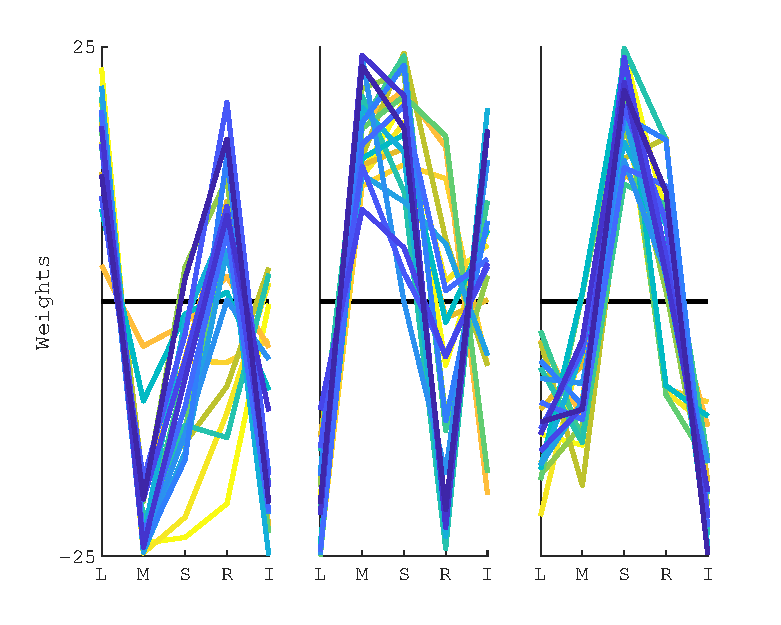
\includegraphics[max width=0.9\textwidth]{figs/LargeSphere/contributions_5.pdf}
\caption{As per Figure \ref{fig:contributions_3} but for the conditions where both rods and ipRGCs were included as additional input signals were considered.} 
\label{fig:contributions_5}
\end{figure}

\begin{figure}[htbp]
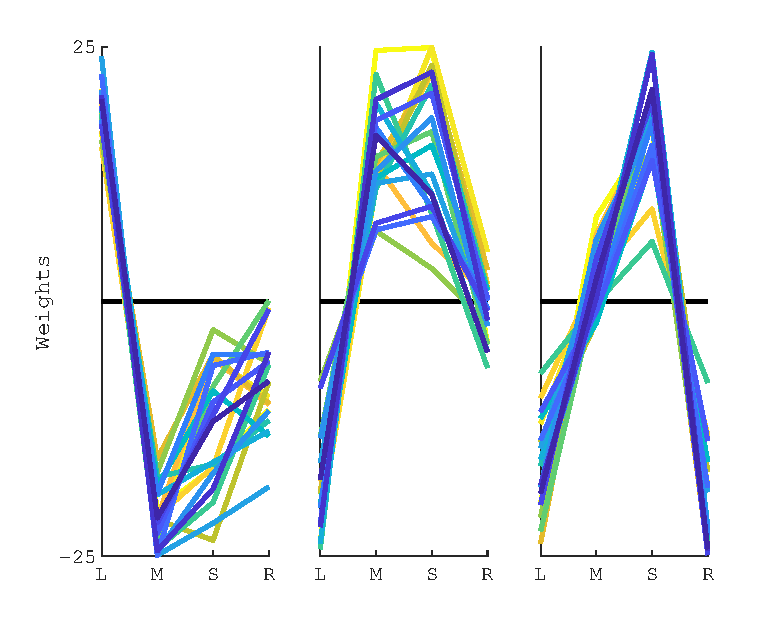
\includegraphics[max width=0.9\textwidth]{figs/LargeSphere/contributions_4.pdf}
\caption{As per Figure \ref{fig:contributions_3} but for the conditions where rods were included as additional input signals.} 
\label{fig:contributions_4}
\end{figure}

\begin{figure}[htbp]
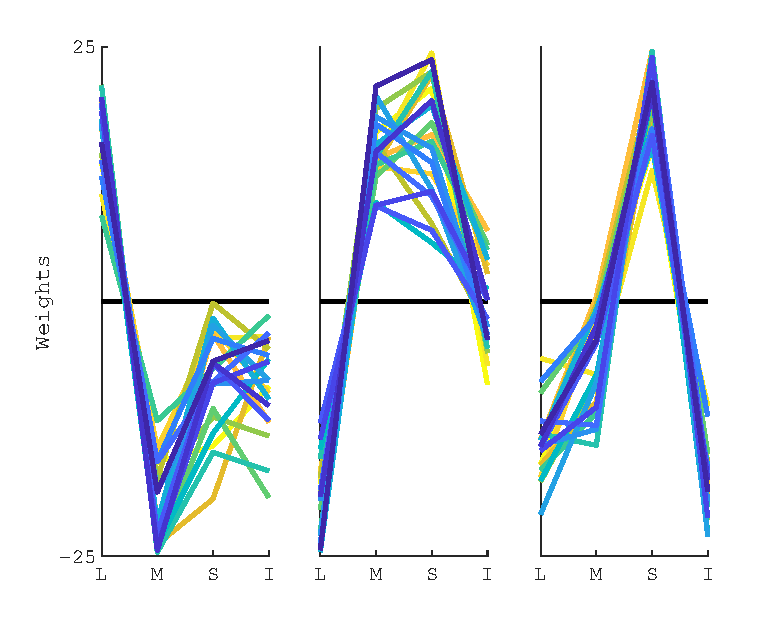
\includegraphics[max width=0.9\textwidth]{figs/LargeSphere/contributions_5minusrods.pdf}
\caption{As per Figure \ref{fig:contributions_3} but for the conditions where ipRGCs were included as additional input signals.} 
\label{fig:contributions_5minusrods}
\end{figure}

Figures \ref{fig:contributions_4} and \ref{fig:contributions_5minusrods} appear somewhat similar. Considering the similar spectral characteristics of rods and melanopsin, it should be expected that the model would use the signals in somewhat similar fashions. It appears as though neither have a particularly strong role to play in the L and M adaptation, however both seem to reliably be used as a negative weighting for S. It is unclear whether this is simply a response to a single high datapoint in this dataset (the peak at 460nm) or whether this integration serves a broader purpose. This peak at 460nm also seems to be the cause for the stubbornly low correlation coefficients for the S channel (compared to L and M), which max out at around 0.81 (see Figure \ref{fig:relcontributions}). 

\clearpage

\section{Conclusion}

Two methods of analysis for the \citet{macdonald_chromatic_2013} data are presented here.

The first analysis \dots

The second analysis showed that the results for one observer could not be well fitted by a simple model of Von-Kries-type observer, but that simple linear combinations of the responses of such an observer could be made to fit the recorded data very well. Though the ability of these fits is to be expected from this type of post-hoc fitting, the types of models which are predicted by the fitting align well with our understanding of post-receptoral signals, which gives us confidence that we may be measuring adaptation at these levels. It would be particularly valuable to see whether the temporal nature of responses also aligned with our understanding of the timecourses of these different signals. 
The second analysis further showed that integration of the simulated rod and melanopic signals provide additional value in fitting the data. Again, this is to be expected from this type of fitting. The minimal improvement delivered by the inclusion of rod and melanopic signals does not furnish me with strong enough evidence to reject the null hypothesis that chromatic adaptation can be fully accounted for by cone and rod mechanisms. 


\subsection{Limitations}

Several limitations have been identified with this experimental design which should be borne in mind when analysing this dataset, or planning similar experiments.

\begin{itemize}
\item How much noise? Repeat sessions.
\item Input imprecision - limits detectable effect sizes.
\item Difficult to say what is biological and what is mechanical.
\item Only trichromatic control, unclear when two effects seems correlated whether it is biological or mechanical.
\item Assumptions about cross-retinal adaptation.
\item Masked by correlation within sessions - difficult to separate. Self - correlation. DG data - following red.
\item Low spectral resolution.
\item Gamut boundary issues.
\end{itemize}


\subsection{Further Work}

The dataset collected by \citet{macdonald_chromatic_2013} may only comprise data from two observers, but it is vastly broad and interesting data which may serve valuable to those interested in chromatic adaptation and colour constancy. Various further analyses are envisioned:
\begin{itemize}
    \item As previously mentioned, there would likely to value in the modelling of the potential response space of an observer on this task, and the interaction the types of analyses performed here.
    \item It would be interesting to consider non-linear adaptation responses. This may better account for the data at the extremes of the wavelength range where luminance was very low.
    \item The temporal dimension of the data is not considered either of the analyses presented here, but the code for the second analysis has been written in such a way that it should be relatively easy to implement. Considering the different expected time courses for adaptation for cones/rods/\glspl{ipRGC} this may serve to be a fruitful avenue.
    \item other observer %%
    \item correct for luminance dependent effects to be able to reduce noise / relax bounds on included data. %%
    \item observers %%
    \begin{itemize}
    \item better observer models incorporating age %%
    \item different observer for central and peripheral %%
    \item sharpened cone spectra - but, careful
    \end{itemize}
\end{itemize}










